% Cap�tulo 2
\chapter{Fundamentação Teórica}
    Ao longo do desenvolvimento do projeto, são usadas peças de hardware essenciais para o funcionamento do robô, nesta seção será apresentado um pouco mais sobre esses componentes e para qual finalidade eles foram usados.

\section{ Arduíno}

O arduíno é utilizado como controle principal do robô. Ele foi criado em 2005 pelo professor Massimo Banzi na Itália. Banzi queria ensinar para seus alunos conceitos de programação e de eletrônica, porém enfrentava um problema, não havia placas de baixo custo no mercado, e portanto isso dificultaria a aquisição do produto por todos os seus alunos. Com isso em mente Banzi decidiu criar uma placa de baixo custo que fosse semelhante a estrutura de um computador para que seus alunos tivessem a oportunidade de aprendizado. A sua placa, nomeada de Arduíno, foi um sucesso, recebendo uma menção honrosa na categoria Comunidades Digitais em 2006. Além disso, foi adotado o conceito de hardware livre, o que significa que qualquer um pode montar, modificar, melhorar e personalizar o arduíno, partindo do mesmo hardware básico. O arduíno é uma placa composta por um microcontrolador Atmel, circuitos de entrada/saída e que pode ser facilmente conectada à um computador e programada via IDE (Integrated Development Environment, ou Ambiente de Desenvolvimento Integrado) utilizando uma linguagem baseada em C/C++, sem a necessidade de equipamentos extras além de um cabo USB. Depois de programado, o microcontrolador arduíno pode ser usado de forma independente.\cite{arduinowiki}

    O arduíno possui uma quantidade enorme de sensores e componentes que podem ser utilizados em vários projetos. Grande parte do material utilizado no arduíno está disponível em módulos, que são pequenas placas que contém os sensores e outros componentes auxiliares como resistores, capacitores e leds. Existem também os chamados Shields, que são placas para serem encaixadas no arduíno para expandir suas funcionalidades. Ao mesmo tempo que permite o acesso do arduíno à uma rede ou até mesmo à internet, mantém os demais pinos disponíveis para utilização, assim pode-se, por exemplo, utilizar os pinos para receber dados de temperatura e umidade de um ambiente, e consultar esses dados de qualquer lugar do planeta.\cite{arduinowiki}
    
    
    Existem vários tipos de  placas que podem ser utilizadas, depende muito do projeto a ser desenvolvido e o número de portas necessárias.
    
    \begin{figure}[htb]
	\centering
  	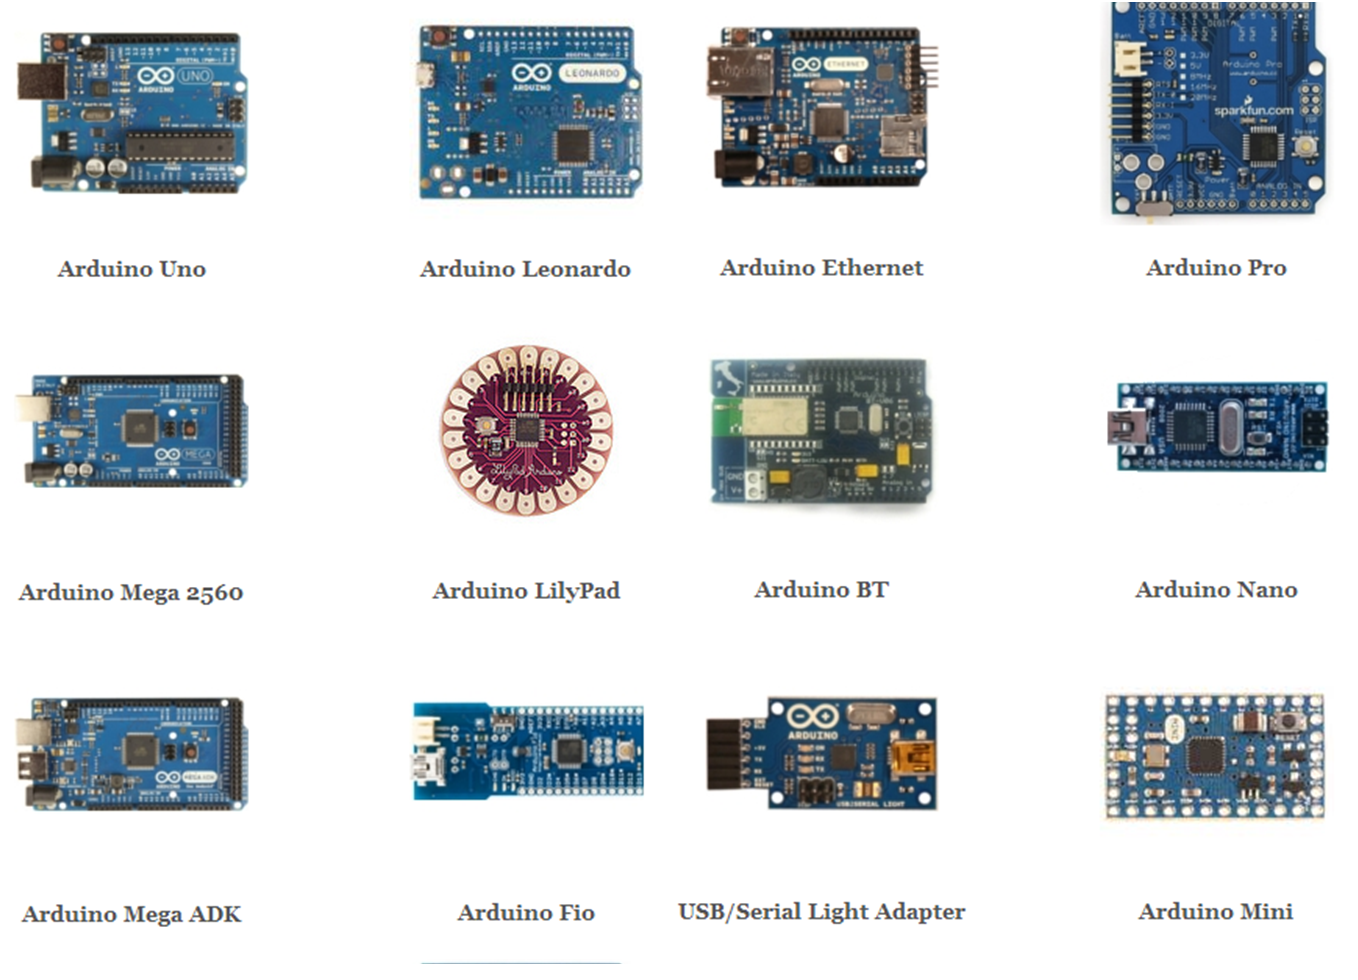
\includegraphics[scale=0.60]{imagens/tipos.png}
  	\textsf{\caption{Tipos de placas da família Arduíno}}
  	\label{fig:FiguraTeste}
\end{figure}
    
    As opções vão das mais comuns, como o arduíno Uno e suas 14 portas digitais e 6 analógicas, passando por placas com maior poder de processamento, como o arduíno Mega, com microcontrolador ATmega2560 e 54 portas digitais, e o arduíno Due, baseado em processador ARM de 32 bits e 512 Kbytes de memória.
    \cite{arduinodetails}
    
    Para o desenvolvimento do projeto usamos o  arduíno Mega, citado anteriormente que pode ser visto na figura abaixo.
    
    \begin{figure}[htb]
	\centering
  	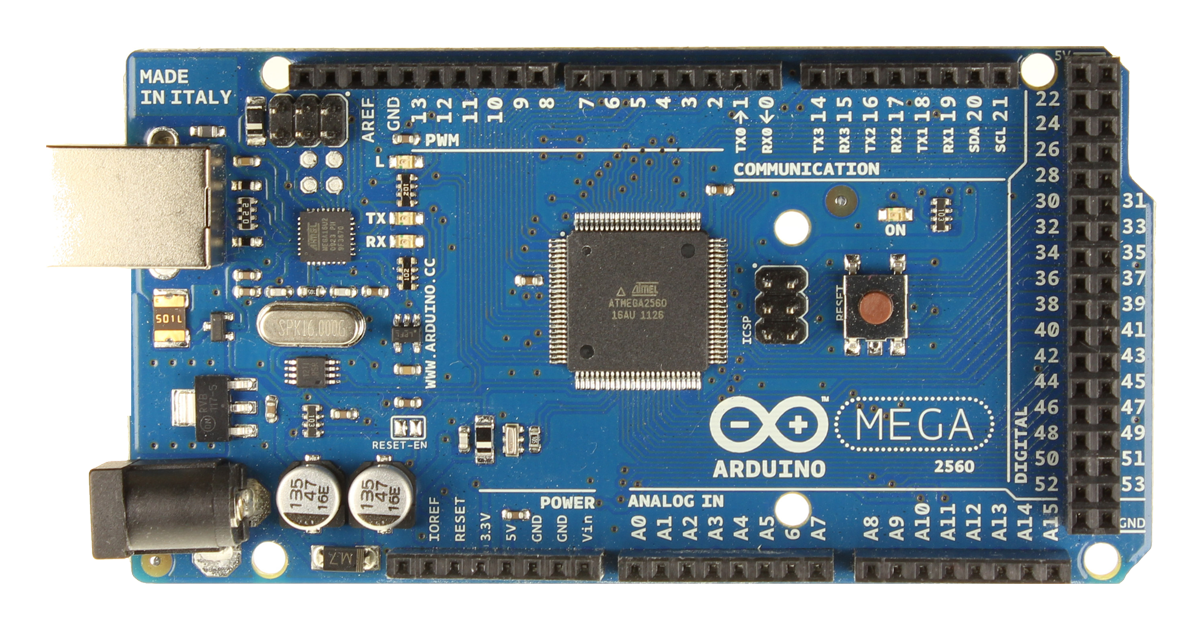
\includegraphics[scale=0.18]{imagens/arduino.png}
  	\textsf{\caption{arduíno Mega}}
  	\label{fig:FiguraTeste}
\end{figure}

    Para programar e passar os comandos para o arduíno, é necessário um programa de software conhecido como IDE.  O arduíno IDE é uma aplicação multiplataforma escrita em Java derivada dos projetos Processing e Wiring. É esquematizado para introduzir a programação a artistas e a pessoas não familiarizadas com o desenvolvimento de software. Inclui um editor de código com recursos de realce de sintaxe, parênteses correspondentes e identação automática, sendo capaz de compilar e carregar programas para a placa com um único clique. Com isso não há a necessidade de editar Makefiles ou rodar programas em ambientes de linha de comando. Tendo uma biblioteca chamada "Wiring", ele possui a capacidade de programar em C/C++. Isto permite criar com facilidade muitas operações de entrada e saída, tendo que definir apenas duas funções no pedido para fazer um programa funcional: setup() – Inserida no início, na qual pode ser usada para inicializar configuração, e loop() – Chamada para repetir um bloco de comandos ou esperar até que seja desligada.\cite{arduinowiki}


\section{Cubo De Rubik}

O cubo de Rubik foi inventado por Ernő Rubik, que foi um conferencista no Departamento de Design Interior na Academia de Artes Aplicadas e Ofícios em Budapeste, Hungria. Ele inventou o  Cubo de Rubik quando estava interessado em geometria, especialmente formas tridimensionais e sua construção. Um dia, enquanto observava o fluxo do Danúbio, Rubik teve a ideia de criar um mecanismo interno cilíndrico que permitisse a manipulação fácil do cubo de 6 faces, cada face dividida em 9 quadrinhos menores, resultando em 54 quadros. Inicialmente achou que seria impossível montar um mecanismo que sustentasse o cubo devido a grande quantidade de movimentos possíveis. Enfim solucionou o problema, e no mesmo ano ganhou o prêmio alemão de "Jogo do Ano" (SpieldesJahres). Em 1985, a SevenTowns comprou os direitos autorais sobre o cubo, reintroduzindo no mercado, obtendo muito sucesso. Atualmente Erno Rubik e SevenTowns trabalham juntos, e Rubik continua sendo o principal beneficiado com sua invenção, estando engajado a descobrir novos quebra-cabeças. Originalmente o cubo de Rubik possui as cores vermelho, laranja, verde, azul, branco e amarelo, mas pode haver variações, de acordo com cada fabricante.\cite{cubohist}

    
    O primeiro cubo de Rubik foi feito de madeira, e hoje o mais comum é encontrá-lo feito de plástico, mas há versões de vidro, papel, entre outras. Ernő Rubik em apenas 31 dias conseguiu solucionar seu quebra cabeça. Hoje em dia o recorde mundial do cubo mágico é de 4.73 segundos pelo Australiano Feliks Zemdegs. O Cubo de Rubik geralmente é confeccionado de plástico, formado por 26 peças e o núcleo distribuídas em 6 faces com cores diferentes. Além do número de peças, suas variações podem ser encontradas em diferentes cores e formatos como, por exemplo, pirâmides, paralelepípedos, e dodecaedro.\cite{cubowiki}
    
       \begin{figure}[htb]
	\centering
  	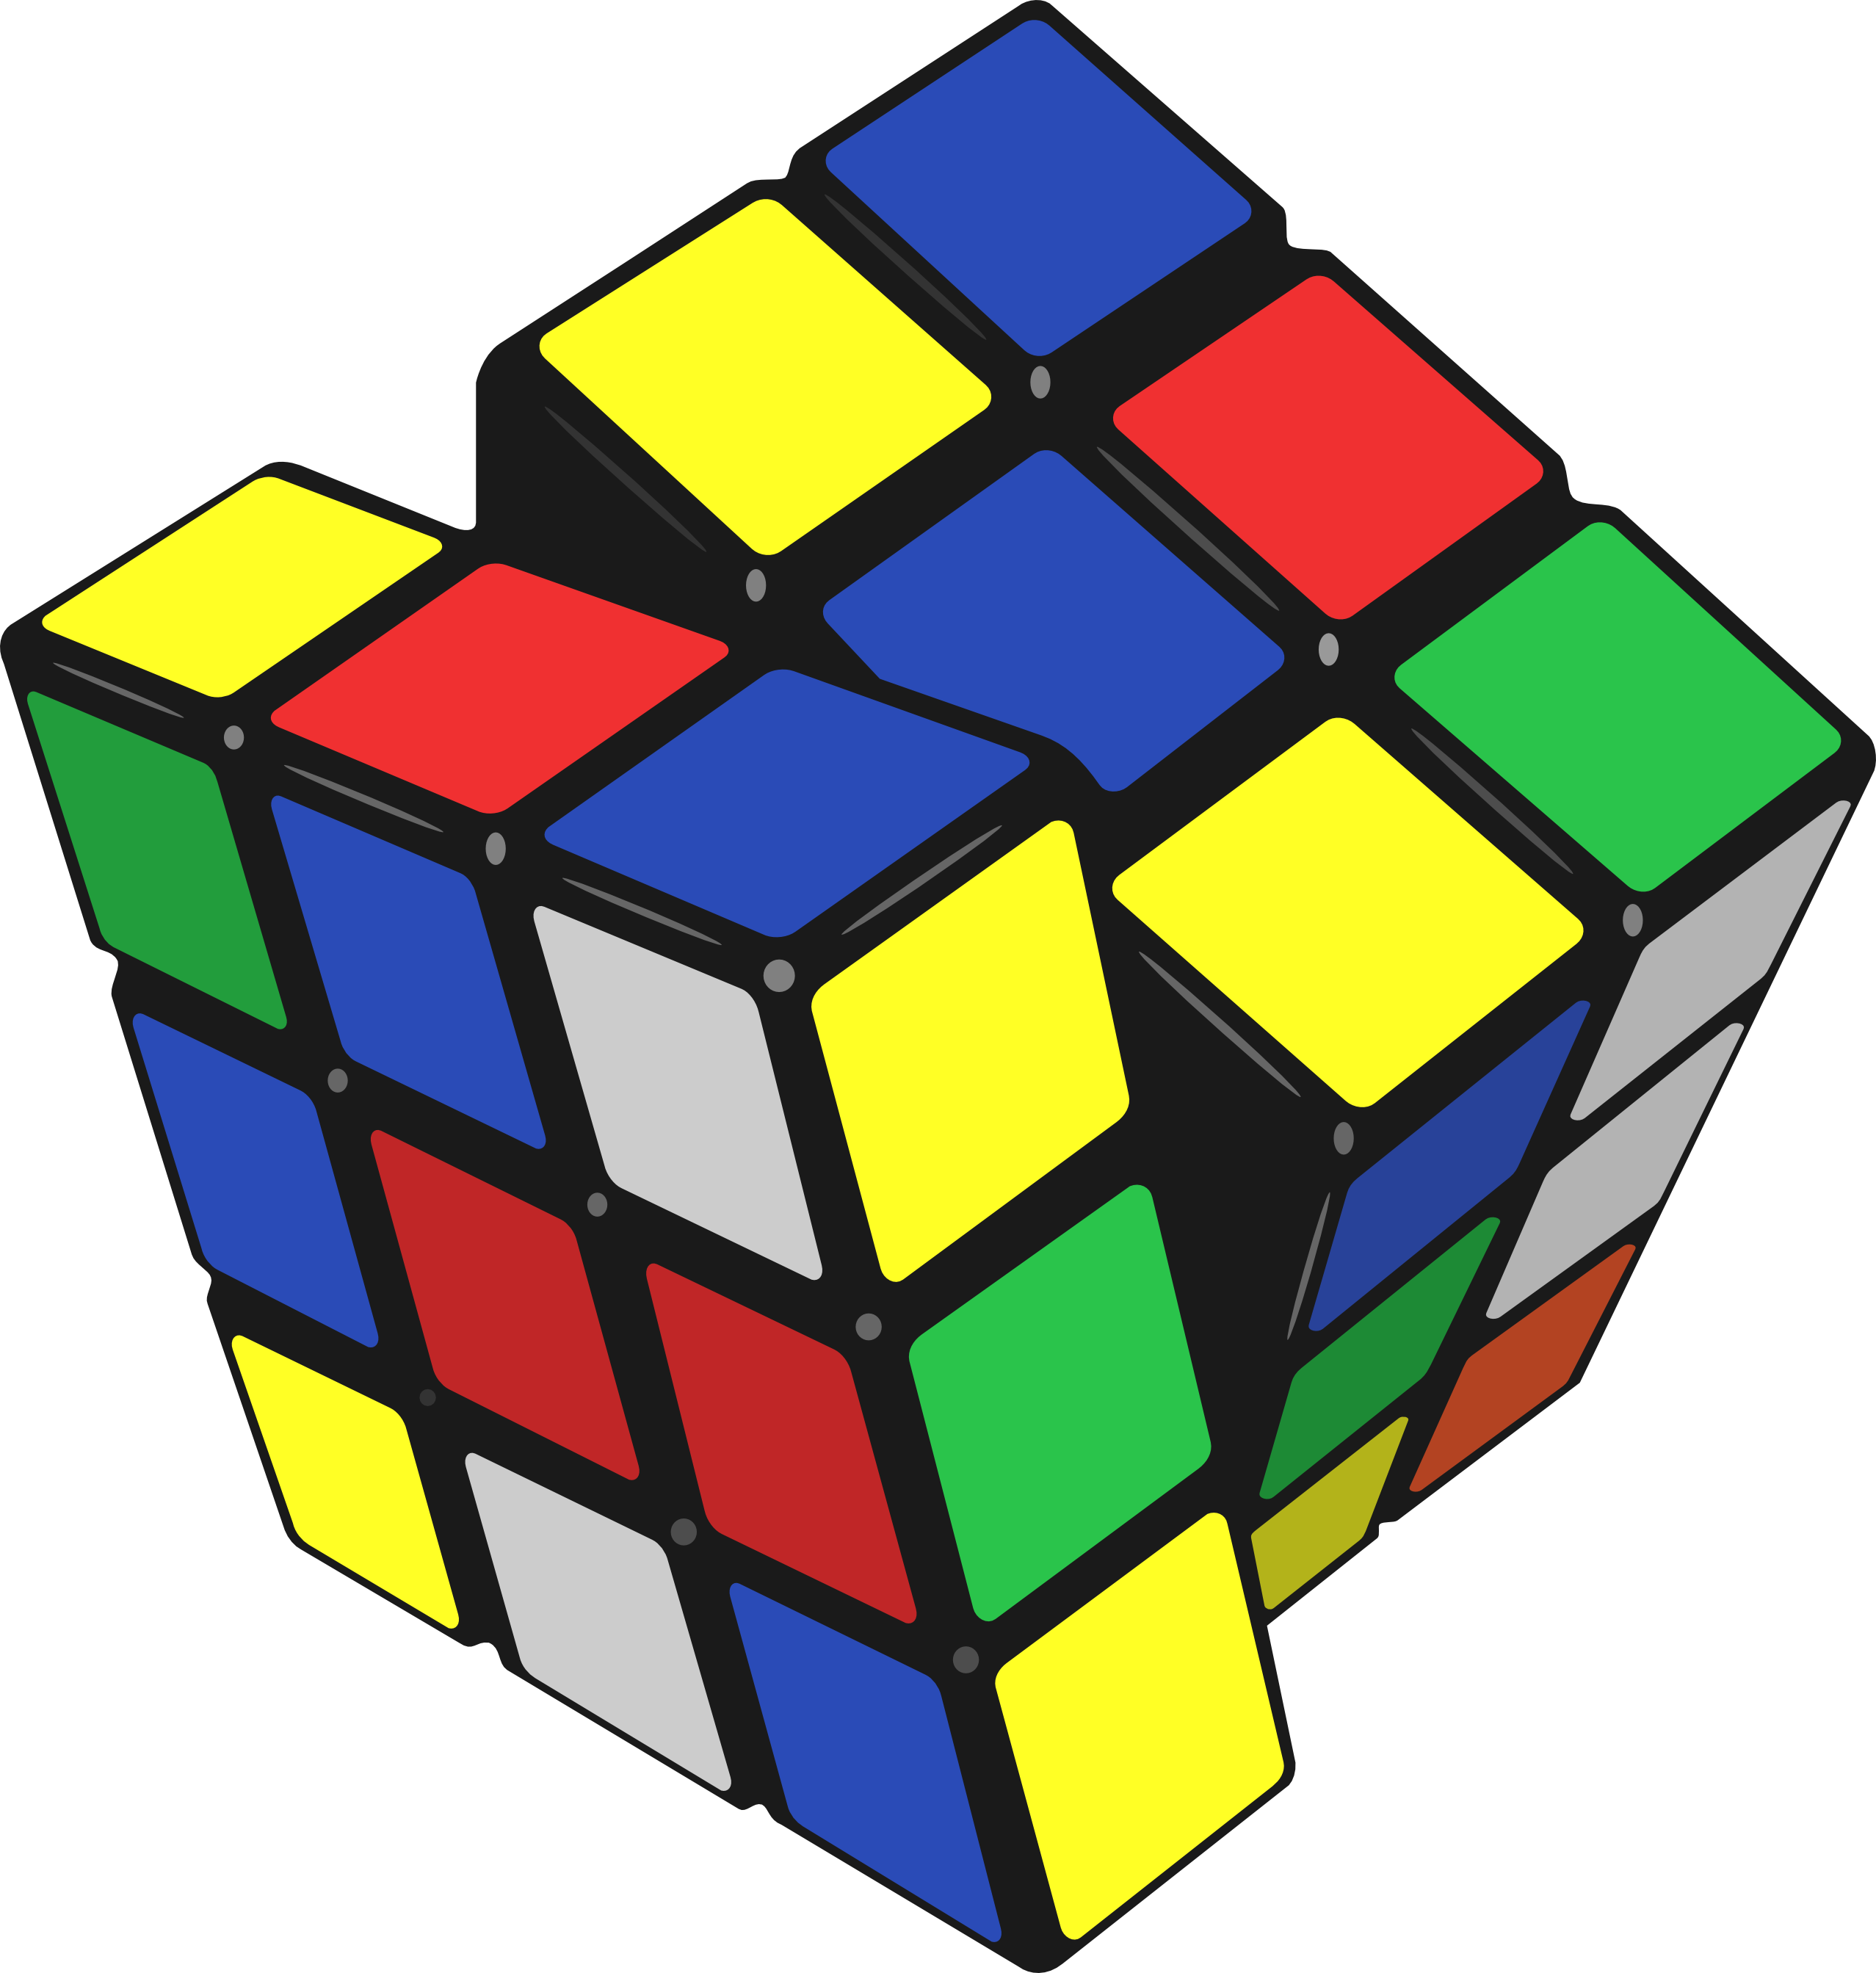
\includegraphics[scale=0.80]{imagens/cubo.png}
  	\textsf{\caption{Cubo de Rubik}}
  	\label{fig:FiguraTeste}
\end{figure}

Calculando todas as configurações possíveis para o cubo mágico, temos um total de aproximadamente 43 quintilhões de combinações diferentes e para realizar todas essas combinações, levaria bastante tempo. Em 2010, Morley Davidson, da Kent StateUniversity, John Dethridge, engenheiro do Google, Herbert Kociemba, professor de matemática da Alemanha, e Tomas Rokicki, programador da Califórnia, com a ajuda dos supercomputadores do Google descobriram que 20 movimentos é o número máximo para resolver qualquer combinação do cubo mágico. \cite{cubociencia}
\section{Bluetooth Arduíno}

Para passar dados e configurações para o robô, é usado um módulo Bluetooth HC-05 que é um módulo MASTER / SLAVE.
Por padrão, a configuração de fábrica é SLAVE. O papel do módulo (mestre ou escravo) pode ser configurado apenas por AT COMMANDS. Os módulos escravos não podem iniciar uma conexão com outro dispositivo Bluetooth, mas pode aceitar conexões. O módulo Mestre pode iniciar uma conexão com outros dispositivos. O usuário pode usá-lo simplesmente para uma substituição de porta serial para estabelecer conexão entre MCU e GPS, PC para o projeto incorporado, etc. O módulo HC-05 é um módulo Bluetooth SPP (Serial Port Protocol) fácil de usar, projetado para configuração de conexão serial sem fio transparente. Como o módulo pode ser usado com as configurações MASTER / SLAVE, se torna uma ótima solução para comunicação sem fio. Este módulo bluetooth de porta serial é totalmente modificado com modulação de 3Mbps de Bluetooth V2.0 + EDR (Enhanced Data Rate) com transceptor de rádio completo de 2,4 GHz e banda base. Ele usa o sistema CSR Bluecore 04-Rocket externo de chip único com tecnologia CMOS e com AFH (Adaptive Frequency Hopping Feature). \cite{bluetooth}

\begin{figure}[htb]
	\centering
  	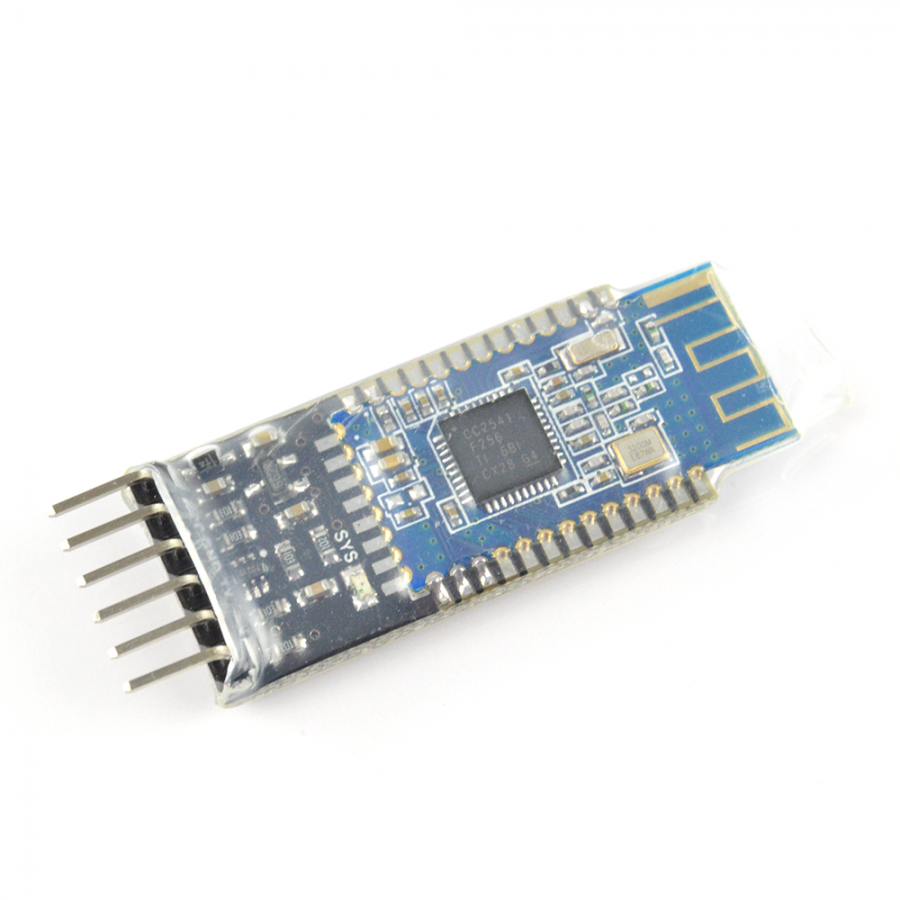
\includegraphics[scale=0.20]{imagens/bluetooh.png}
  	\textsf{\caption{Bluetooth Arduíno}}
  	\label{fig:FiguraTeste}
\end{figure}

    O Módulo Bluetooth HC-05 possui 6 pinos. Eles são os seguintes:
    
     \begin{itemize}
       \item Habilitar: 
    Quando a habilitação é puxada LOW, o módulo está desabilitado, o que significa que o módulo não liga e falha em comunicar. Quando o habilitação é deixada aberta ou conectada a 3.3V, o módulo está habilitado, e o módulo permanece ligado e a comunicação também ocorre.
       \item Vcc: tensão de alimentação 3.3V a 5V.
       \item GND: pino de terra.
       \item TXD e RXD: esses dois pinos atuam como uma interface UART para comunicação.
       \item Estado: atua como um indicador de status. Quando o módulo não está conectado a nenhum outro dispositivo bluetooth, o sinal fica baixo. Neste estado baixo, o led pisca continuamente o que indica que o módulo não está emparelhado com outro dispositivo. Quando este módulo está conectado ou emparelhado com qualquer outro dispositivo bluetooth, o sinal vai alto. Neste estado alto, o led pisca com um atraso constante, por exemplo, o atraso 2 segundos que indica que o módulo está emparelhado.
       \item Switch do botão: usado para alternar o módulo no modo de comando AT. Com a ajuda dos comandos AT, o usuário pode alterar os parâmetros deste módulo, mas somente quando o módulo não está emparelhado com qualquer outro dispositivo BT. Se o módulo estiver conectado a qualquer outro dispositivo bluetooth, ele começa a se comunicar com esse dispositivo e não funciona no modo de comando AT.
     \end{itemize}\cite{bluetooth}


\section{Trabalhos Relacionados}

Nesta seção, será apresentado alguns robôs que também foram desenvolvidos para solucionar o problema do cubo de Rubik.

\subsection{Tilted Twister 2.0}

  \begin{figure}[htb]
	\centering
  	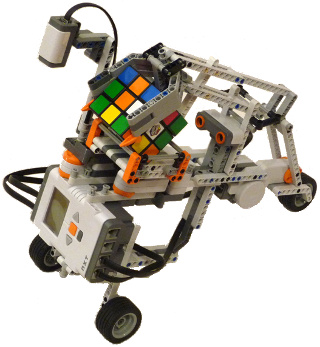
\includegraphics[scale=0.25]{imagens/tiltedtwister2.jpg}
  	\textsf{\caption{Tilted Twister 2.0}}
  	\label{fig:FiguraTeste}
\end{figure}

O Tilted Twister 2.0, como foi nomeado, é um robô que soluciona o cubo de Rubik usando o conjunto LEGO Mindstorms NXT 2.0. Ele resolve um cubo de Rubik padrão, sendo completamente autônomo e funciona sem a ajuda de um computador. Para detectar as cores, utiliza o sensor de cor LEGO Mindstorms e para  resolução do cubo,  usa o algoritmo de Duas Fases de Herbert Kociemba.\cite{robo1}

O criador do robô, Hans Andersson, afirma que mesmo que o sensor de cor LEGO Mindstorms seja muito preciso, é difícil distinguir entre as cores vermelha e a laranja pois existe uma redundância na medida em que é possível usar as cores de dois lados para determinar a cor do terceiro. Os cubos centrais têm ainda mais redundância. Ele relata também que a única coisa para se considerar era o logotipo do Rubik na peça central branca, que fornece leituras de cores indefinidas. A primeira parte implementada do algoritmo do robô foi o método de canto-primeiro, que gera uma solução razoavelmente curta. A média é de cerca de 60 voltas faciais. O programa calcula três soluções com diferentes pontos de partida e escolhe o menor.\cite{robo1}

\subsection{CubeStormer II}

Um robô feito de peças de Lego e com o cérebro fornecido por um smartphone conseguiu resolver o cubo de Rubik em pouco mais de cinco segundos. De acordo com a edição norte-americana do site Gizmodo, a máquina, chamada de CubeStormer II, criada por David Gilday e Mike Dobson, resolveu o quebra-cabeça em 5.352 segundos. O recorde anterior era do australiano Felils Zemdegs(um ser humano) com o tempo de 5.66 segundos que foi registrado pelo Guinness.\cite{robo2}

\begin{figure}[htb]
	\centering
  	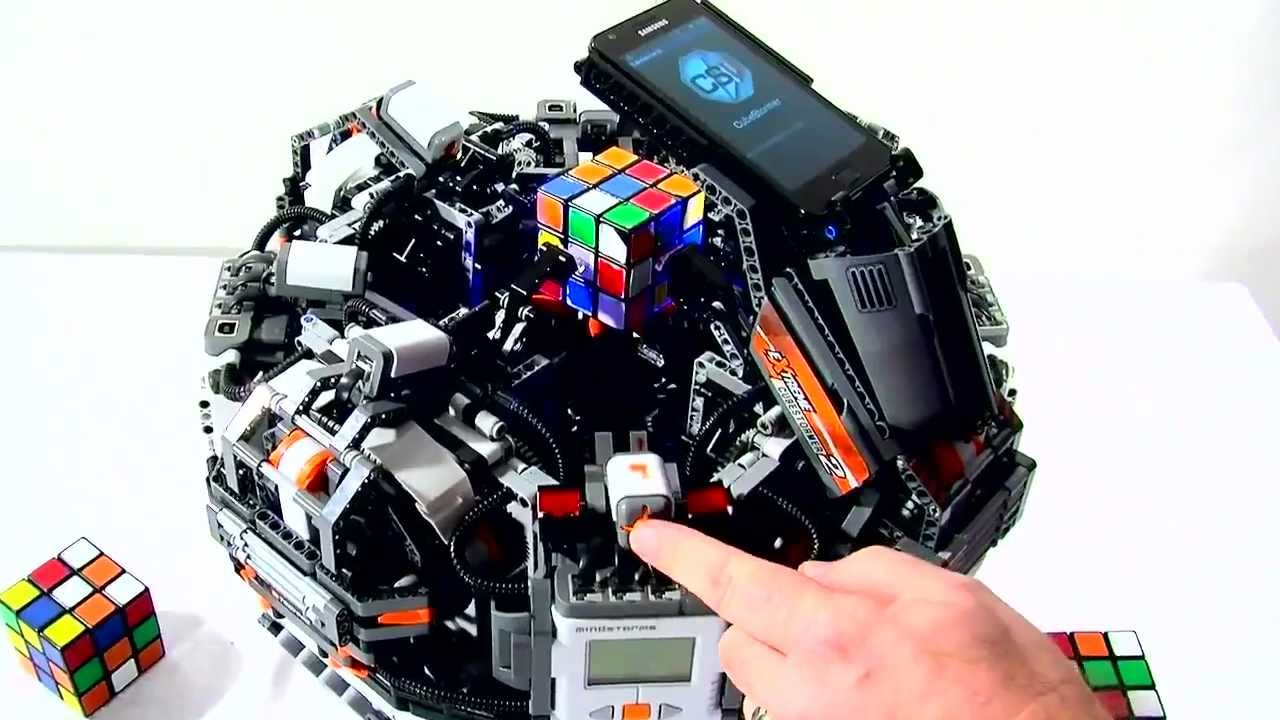
\includegraphics[scale=0.25]{imagens/storm.jpg}
  	\textsf{\caption{CubeStormer II}}
  	\label{fig:FiguraTeste}
\end{figure}


    O robô utiliza a câmera do celular para capturar imagens de cada lado do cubo e as analisa. Em seguida, envia as instruções por meio da conexão sem fio Bluetooth para os braços da máquina que rodam e resolvem o quebra-cabeça em alta velocidade.\cite{robo2}


\subsection{Sub1 Reloaded}

\begin{figure}[htb]
	\centering
  	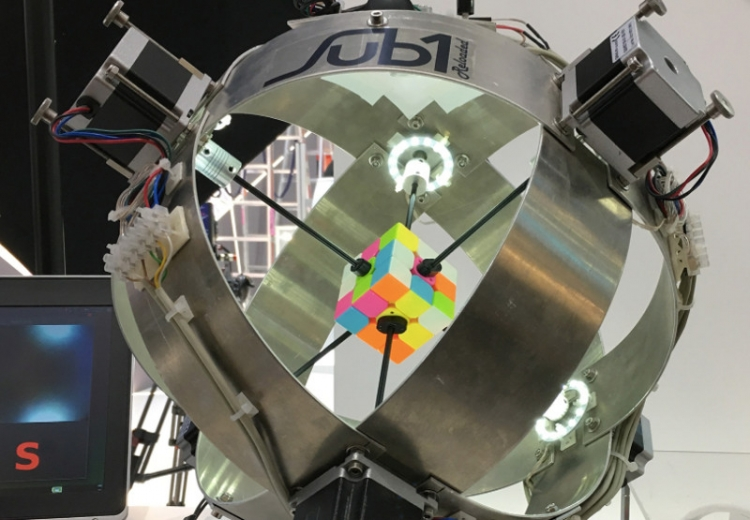
\includegraphics[scale=0.30]{imagens/sub.jpg}
  	\textsf{\caption{Sub1 Reloaded}}
  	\label{fig:FiguraTeste}
\end{figure}

O engenheiro alemão Albet Beer desenvolveu um robô que conseguiu resolvem o cubo mágico em 0,637 segundo, batendo seu próprio recorde mundial, segundo o Livro Guinness de Recordes. O robô Sub1 Reloaded tem um novo processador Infineon e é composto de uma câmera que "enxerga" o cubo. Uma vez achada a solução, seis braços mecânicos resolver o quebra-cabeças, em exatamente 21 movimentos. O recorde anterior, de janeiro de 2016, era de 0,887 segundos mas um novo recorde foi estabelecido na feira electrónica, na cidade alemã de Munique, no fim de 2016, e reconhecido agora pelo Guinness.\cite{robo3}

Agora conhecido como Sub1 Reloaded, o robô raspou mais de um quarto de seu tempo recorde de 2016 de 0,887 segundos depois de receber um novo processador Infineon. O processo de resolver o enigma começa quando um computador recebe duas fotos do Cubo de Rubik, e em seguida, identifica a cor de cada peça e usa a implementação de Tom Rokicki do algoritmo de duas fases de Herbert Kociemba para determinar a solução mais rápida. Uma placa de microcontrolador Infineon AURIX compatível com arduíno opera então os seis braços mecânicos do robô, permitindo que ele complete o quebra-cabeça em 21 movimentos.\cite{robo3}

\subsection{O Robô de Jay Flatland e Paul Rose}

\begin{figure}[htb]
	\centering
  	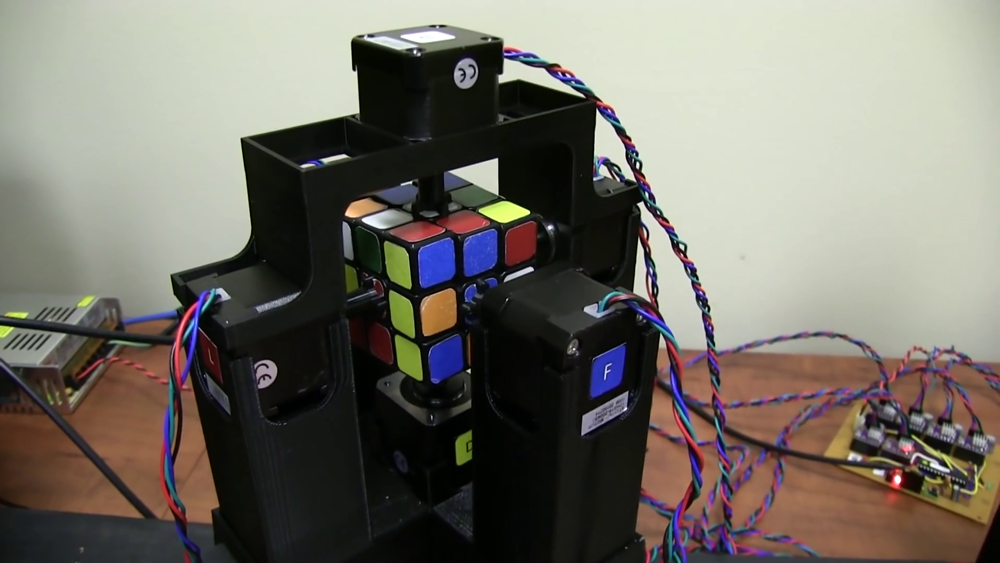
\includegraphics[scale=0.25]{imagens/roboresolverkubrik.jpg}
  	\textsf{\caption{Robô de Jay Flatland e Paul Rose}}
  	\label{fig:FiguraTeste}
\end{figure}

    Dois engenheiros de software criaram um robô capaz de resolver o cubo mágico em questão de instantes. Jay Flatland e Paul Rose desenvolveram uma máquina que resolveu o cubo de Rubik em 1,196 segundos, mas em algumas tentativas, o robô demorou apenas 1,047 segundos. O robô que foi construído é composto por componentes produzidos com o auxílio de uma  impressora 3D, por webcams e por um chip arduíno, que transmite informação acerca das cores das  faces coloridas do cubo para um computador. Este equipamento utiliza o sistema Linux, juntamente com um algoritmo chamado Kociemba para resolver os puzzles.\cite{robo4}
    
    A ideia principal do algoritmo de Kociemba é definir um objetivo intermediário e resolver o problema em dois passos, ou seja, pegar um cubo completamente embaralhado, encontrar uma sequência de movimentos que o coloque num subconjunto especial do espaço de busca e, finalmente, resolve-lo.\cite{robo4}

